\documentclass[tikz,border=10pt]{standalone}
\usepackage{tikz}

\begin{document}

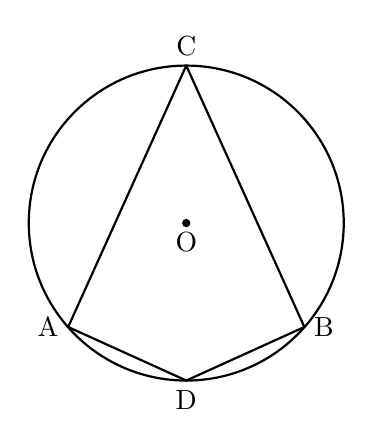
\begin{tikzpicture}[scale=1, line cap=round, line join=round]

% Center
\coordinate (O) at (0,0);
\fill (O) circle (1.5pt);

% Draw Circle
\draw[thick] (O) circle (2);

% Points on the circumference
\coordinate (C) at (0,2);
\coordinate (D) at (0,-2);
\coordinate (A) at (-1.5,-1.32);
\coordinate (B) at (1.5,-1.32);

% Draw Quadrilateral ACDB
\draw[thick] (C) -- (A) -- (D) -- (B) -- cycle;

% Labels
\node[below] at (O) {O};
\node[above] at (C) {C};
\node[below] at (D) {D};
\node[left] at (A) {A};
\node[right] at (B) {B};

\end{tikzpicture}

\end{document}
